\documentclass[9pt,oneside]{amsart}

% -------------------------------------------------------------------------------
% Packages
% -------------------------------------------------------------------------------

\usepackage[a4paper,width=170mm,top=18mm,bottom=22mm,includeheadfoot]{geometry}
\usepackage[us,12hr]{datetime} % `us' makes \today behave as usual in TeX/LaTeX
\usepackage[usenames,dvipsnames]{xcolor}
\usepackage{multicol,caption}
\usepackage{url}
\usepackage{xspace}
\usepackage{cancel}
\usepackage{graphicx}
\usepackage{subfig}
\usepackage{amsmath}
\usepackage{amssymb}
\usepackage{textcomp}
\usepackage{booktabs}
\usepackage{array}
\usepackage{verbatim}
\usepackage{caption}
\usepackage{cite}
\usepackage{float}
\usepackage{pdflscape}
\usepackage{mathtools}
\usepackage{romannum}
\usepackage{afterpage}
\usepackage{multido}
\usepackage{color}
\usepackage{background}
\usepackage{witharrows}
\usepackage{lipsum}
\usepackage{booktabs}
\usepackage{siunitx}
\usepackage{tikz}
\usepackage{tikzit}
\input{nodes.tikzstyles}

\newcolumntype{C}[1]{>{}m{#1}}
\renewcommand\tabularxcolumn[1]{C{#1}}

% -------------------------------------------------------------------------------
% Paper Style
% -------------------------------------------------------------------------------

\unitlength=1mm
\definecolor{lightyellow}{rgb}{1,0.99,0.95}
\usetikzlibrary{decorations.markings,calc}

\DeclarePairedDelimiter{\ceil}{\lceil}{\rceil}

\newenvironment{Figure}
  {\par\medskip\noindent\minipage{\linewidth}}
  {\endminipage\par\medskip}

\def\Toty{60}   %% adjust
\def\Totx{55}   %% adjust
\def\Offy{0.3}

\pagecolor{orange}

\newsavebox{\mybox}
\sbox{\mybox}{%

\begin{tikzpicture}[remember picture]
  \foreach \y in {1,2,...,\Toty}{
    \foreach \x in {2,4,...,\Totx}{
        % Time permitting create paw prints
        % \fill[\Dotcolor,shift={(\Stepx*\x cm,\Stepy*\y cm)}] (0,) circle[radius=\Size];
   }%
    \foreach \x in {1,3,...,\Totx}{
        % Time permitting create paw prints
        % \fill[\Dotcolor,shift={(\Stepx*\x cm,\Offy cm+\Stepy*\y cm)}] (0,) circle[radius=\Size];
   }%
   }%
\end{tikzpicture}
 }%

\backgroundsetup{
 scale=1, angle=10, position={current page.center}, contents={%

\begin{tikzpicture}[remember picture,overlay]
    % \node at (current page.center) {\usebox\mybox};
\end{tikzpicture}%
 }%
}%

\providecommand{\tightlist}{%
  \setlength{\itemsep}{0pt}\setlength{\parskip}{0pt}}

% -------------------------------------------------------------------------------
% Custom commands
% -------------------------------------------------------------------------------
 
\newcommand{\hcancel}[1]{%
  \tikz[baseline=(tocancel.base)]{
    \node[inner sep=0pt,outer sep=0pt] (tocancel) {#1};
 %   \draw[black] (tocancel.south west) -- (tocancel.north east);
   }%
 }%

\newcommand{\inputTikZ}[2]{%  
     \scalebox{#1}{\input{#2}}  
}

\newcommand*\eg{e.g.\@\xspace}
\newcommand*\Eg{e.g.\@\xspace}
\newcommand*\ie{i.e.\@\xspace}

\newcommand{\RNum}[1]{\uppercase\expandafter{\romannumeral #1\relax}}
\newcommand*\compu{COMPU\textsuperscript{\texttrademark}GLOBAL\textsuperscript{\texttrademark}HYPER\textsuperscript{\texttrademark}MEGA\textsuperscript{\texttrademark}CORP\textsuperscript{\texttrademark}}
\newcommand*\proofmeow{PROOF OF MEOW\textsuperscript{\textregistered}}
\newcommand*\lipsumeow{Meow, meow, meow, meow, meow, meow, meow, meow.  Meow, meow, meow. Meow, meow, meow, meow, meow, meow, meow, meow. Meow, meow, meow, meow, meow, meow, meow, meow. }
\newcommand*\lipsumeowpurr{Purr. meow, puuuuurrrr, mrrowwwwrrrrrr, meow, meow, meow. Meow, meow, meow, meow, meow, meow, meow, meow. Meow, meow, meow, meow, meow, meow, meow, meow. Meow, meow, meow, meow, meow, meow, meow, meow. Mrow, mrrr, prrr, mrrrrrrrrwwwwrrrrrr. Meow, meow, meow, meow, meow, meow, meow, meow.}
\newcommand*\lipsumhiss{Meow, hiiiiiiiiissssssssssss, meeeeeeeewwwwwr, mrrrroworroror, meow.}

\newcommand*\datetimenow{\THEYEAR\THEMONTH\THEDAY\currenttime}

% -------------------------------------------------------------------------------
% Title/Author
% -------------------------------------------------------------------------------

\title{\RNum{2020} \compu{} \\ Architecture and Protocol\\ for Proof of Meow\textsuperscript{\textregistered}\\ {\smaller{\textbf{(Draft 1.0.5)}}}}
\author{Mr. [Redacted] Whiskers}

% -------------------------------------------------------------------------------
% Preamble Concluded
% -------------------------------------------------------------------------------

\begin{document}

\begin{abstract}
 A number of consensus protocols have emerged after Satoshi Nakomoto proposed Proof of Work \cite{nakamoto2009bitcoin}. However, Proof of Stake models have emerged as both computationally more efficient with economic incentives to protect against bad actors. We propose \proofmeow{} which is not only computationally efficient but cute too. Below we describe the protocol, demonstrate mathematically its superiority over conventional schemes, and describe the World Domination Meow Token offering under the symbol CAT.
\end{abstract}

\maketitle

\setlength{\columnsep}{20pt}
\begin{multicols}{2}

% -------------------------------------------------------------------------------
% Keywords/Terminology
% -------------------------------------------------------------------------------

\section{Kittywords}\label{sec:keywords} {blockchain, cryptocurrency, permission-ed networks, proof of stake, proof of work, high-speed transactions, decentralized application, dApp, smart contract, distributed crypto-exchange service}, know your customer, anti-money laundering, \meow{}

\section{Termeowology}\label{sec:terminology}
\begin{description}
    
    \item[Byzantine Meow-eneral consensus problem] describes a situation in which, in order to avoid catastrophic failure of the system, the system's actors must agree on a concerted strategy, but some of these actors are unreliable.
    
    \item[Cryptokitties] Virtual kitties based on the ERC-721 protocol which demonstrated the most important function of Ethereum, and perhaps all peer-to-peer networks, including blockchain ledgers.
    
    \item[dApp] Decentralized application, a term coined by Ethereum, is a back-end service application that operates on a peer-to-peer network without a centralized server.
    
    \item[Distributed crypto-exchange service] A cryptocurrency exchange service utilizing smart contracts to maximize security and transparency of the exchange operation.
    
    \item[Peer-to-peer, p2p] Peer-to-peer computing or networking is a distributed application architecture that partitions tasks or workloads between peers. Peers are equally privileged, equipotent participants in the application. They are said to form a peer-to-peer network of nodes.
    
    \item[Smart contract] A smart contract is a computer protocol intended to digitally facilitate, verify, or enforce the negotiation or performance of a contract. Smart contracts allow the performance of credible transactions without third parties. These transactions are trackable and irreversible.
    
    \item[Proof of Meow\textsuperscript{\textregistered}] A new consensus mechanism which primarily revolves around being cute.
\end{description}

\section{Introducing Mr. Whiskers}\label{sec:whiskers}
\begin{Figure}
    \medskip
    \centering
%    
\includegraphics[width=0.80\textwidth]{figures/mrwhiskers.png}
    
\includegraphics[width=0.80\textwidth]{figures/mrwhiskerstokenme.png}
    \captionof{figure}{"Meow, meow, meow" said Mr. Whiskers being super cute.}
    \medskip
\end{Figure} 

% -------------------------------------------------------------------------------
% Preface
% -------------------------------------------------------------------------------

\section{Purreface}\label{sec:preface}
 This is intended to be a technical ``vision'' summary of one possible direction that may be taken in further developing the \meow{} ecosystem with some rationale as to why this direction is awesome. It lays out in virtually no detail except trying to be cute.

 It is not intended to be relied upon for foreword looking statements or any investment decisions. It is not intended to be a specification, formal or otherwise. 

 The appendix contains as many disclosures as we could reasonably finds and collate which were applicable to this paper and our intentions.

% -------------------------------------------------------------------------------
% Version History
% -------------------------------------------------------------------------------

\subsection{Version Hisstory}\label{subsec:history}

\begin{itemize}
 \item 09/28/2019: 1.0.0
 \item 09/29/2019: 1.0.5-bib
\end{itemize}

\subsection{Compilation Time}\label{subsec:compilation}

 \textit{{\ddmmyyyydate\today} at \currenttime}

% -------------------------------------------------------------------------------
% Background
% -------------------------------------------------------------------------------

\section{Catground}\label{sec:background}
 \lipsumeow{} 
 Classically, meow, meow, purr, hiss, meow, meow, merrorrrrow.

\begin{enumerate}
 \item Meow (m) Meow, meow, meow. (m)
 \item Hiss (h) Hiss, hiss, meow. (h)
 \item Purr (p) Purr, hiss, meow. (p)
\end{enumerate}

\begin{equation}
\psi_{p,h}^{n+1}=\frac{1}{4}\left( \psi_{p+1,h}+\psi_{p-1,h}+\psi_{p,h-1}+\psi_{p,h+1}\right)\;\;
\label{subsec:mrwhiskers}
\end{equation}

\section{Meowrchitecture}\label{sec:architecture}
 
 \lipsumeow{}
 
\begin{enumerate}
  \item Meow 
  \item Purr
  \item Mewwor
  \item Hiss
\end{enumerate}

\subsection{Networkitty Topology}\label{subsec:network_topology}

 \lipsumeow{} Proof of Meow.\textsuperscript{\textregistered} Catsensus protocols. Buzzwords. Meow:
 
\begin{itemize}
 \item \textbf{Meow}  Meow, meeeeooowrr.
 \item  \textbf{Meow, meow} \lipsumeow{}
 \item  \textbf{Meow, hiss, meow} \lipsumhiss{}
 \item  \textbf{Meow, hiss, purr} \lipsumeowpurr{}
\end{itemize}
 
\subsection{Meow, purr, hiss, meow.}\label{subsec:decentral_security_scalable}

\begin{enumerate}
   \item Meow, purr, hiss, meow
       \begin{enumerate}
          \item Meow, meow
          \item Meow, purr, meow
          \item Meow, hiss, meow
          \item Purr, meow, purr
          \item Purr, meow, hiss
          \item Hiss, meow, purr
          \item Hiss, purr, hiss
          \item Hiss, hiss, hiss
       \end{enumerate}  
   \item Hiss, purr, purr
       \begin{enumerate}
          \item Meow, meow, meow (m)
          \item Purr, purr, meow (p)
          \item Hiss, hiss, meow (h)
       \end{enumerate}
\end{enumerate}
 
Meow, meow, meow. Hiss, hiss, hiss. Purr, purr, meow. \textit{Meow-chain}.  

\begin{Figure}
    \medskip
    \centering
    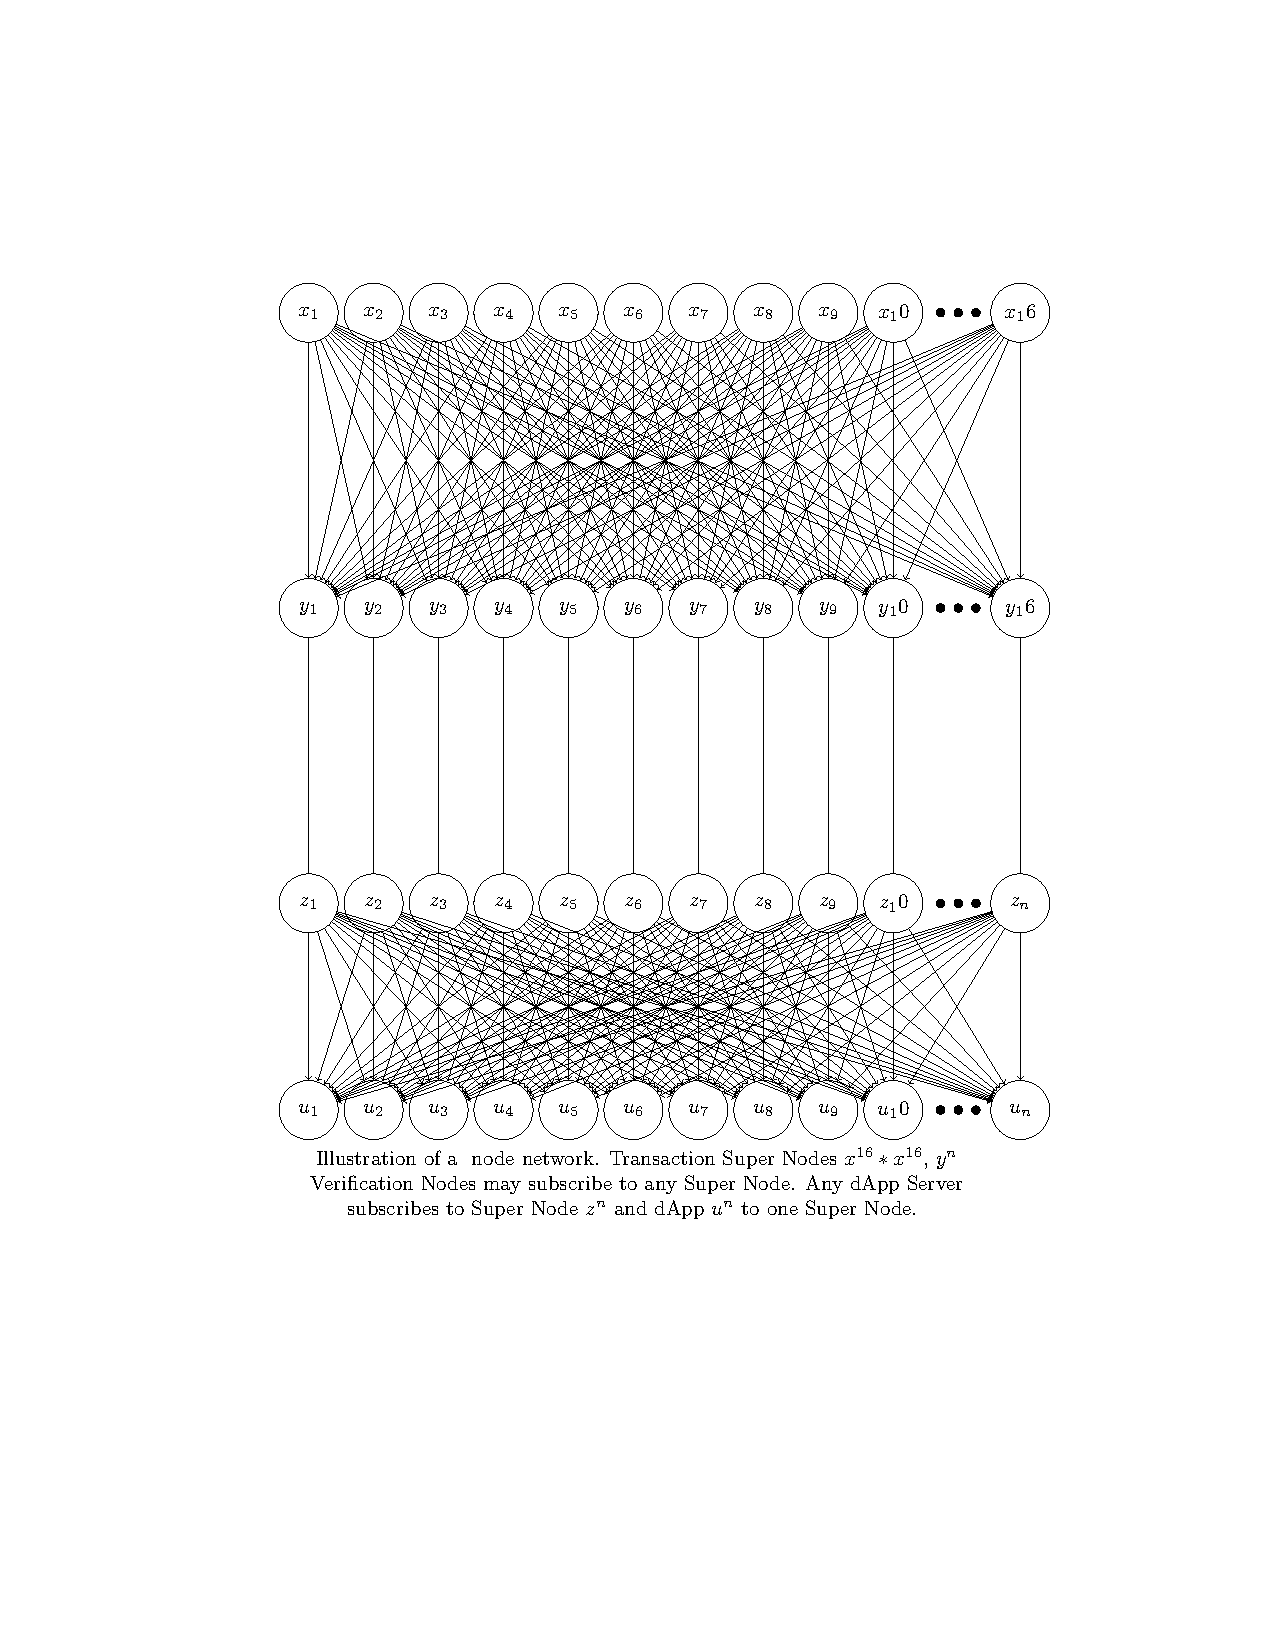
\includegraphics[width=0.95\textwidth]{figures/figure_1_cropped.pdf}
    \captionof{figure}{Meow, meow, meow communications.}
    \medskip
\end{Figure}

Kitty points are:

\begin{itemize}
    \item \lipsumeowpurr{}
    \item \lipsumhiss{}
    \item \lipsumeow{}
\end{itemize}

Proof-of-Meow\textsuperscript{\textregistered}:

\begin{proof}
  Let $purr,hiss \in \mathbb{R}$ where $purr=xy$ and $hiss=z(meow)$. So,
  \begin{DispWithArrows*}
    4xyzw &= 2\cdot2purr(hiss) \\
    &\le 2\cdot(purr^2+hiss^2) \Arrow[i]{substituting meow-riables}\\
    &= 2\cdot((xy)^2+(z(meow))^2)  \\
    &= 2\cdot(x^2y^2+z^2meow^2) \\ 
    &= 2x^2y^2+2z^2meow^2 \\
    &\le ((x^2)^2+(y^2)^2)+((z^2)^C2)+(meow^2)^2) \\
    &= x^4+y^4+z^4+w^4 \qedhere
  \end{DispWithArrows*}
\end{proof}

The advantages of this meowrchitecture are:

\begin{itemize}
    \item \textbf{Meow, hiss, purr} \lipsumeow{}
    \item \textbf{Purr, hiss, meow} \lipsumeowpurr{}
    \item \textbf{Hiss, purr, meow} \lipsumhiss{}
\end{itemize}

As a result: \\


% \centering
\textit{Problems in Classical Computing are Meow-able} \\
\begin{tabular}{ |p{2.2cm}|p{3cm}|p{2.2cm}| }
     \hline
     \begin{center}\textbf{\textit{Mathematical Notation}}\end{center} & \begin{center}\textbf{\textit{Catplexity\\ Time}}\end{center} & \begin{center}\textbf{\textit{Tracatable/\\Intracatable}}\end{center}\\
     \hline
     \textbf{O(k$^{n}$), O(2$^{n}$)} & Exponential & \textbf{Meowable} \\
     \hline
     \textbf{O(n!)} & Factorial & \textbf{Meowable} \\
     \hline
     \textbf{O(n$^{n}$)} & Super-Exponential & \textbf{Meowable} \\
     \hline
\end{tabular}

\subsection{Meow, purr, hiss, meow protocol}\label{subsec:meow}

 \lipsumeow{}
 \\
 \lipsumeowpurr{}
 
\textit{Meow, meow, meow and meow communications}.  

% -------------------------------------------------------------------------------
% Figure PDF
% -------------------------------------------------------------------------------

\begin{Figure}
    \medskip
    \centering
    \ctikzfig{meow-hiss-purr_2}
    \captionof{figure}{Meow, meow, meow consensus.}
    \medskip
\end{Figure}

Key points are:

\begin{itemize}
    \item Meow, meow, purr
    \item Meow, meow, hiss, purr, meow
    \item Meow, purr, hiss, meow
\end{itemize}


 This Figure shows the relationship meow and purr. 

% -------------------------------------------------------------------------------
% Figure PDF
% -------------------------------------------------------------------------------

\begin{Figure}
    \medskip
    \centering
    \ctikzfig{network_figure}
    \captionof{figure}{Meow, hiss, purr.}
    \medskip
\end{Figure}

\subsection{\proofmeow{} Subsection with financials}\label{subsec:financials_3}

% -------------------------------------------------------------------------------
% Allocation of Tokens
% -------------------------------------------------------------------------------

\subsubsection{\compu{} Spreadsheet}\label{subsec:spreadsheet}

The \textit{Compu} World Domination Meow Token or \proofmeow{}-coins will issue \textbf{10,000,000,000} meow-coins, with an initial offer price of \textbf{\$0.01} per token.  Out of which:
\\
\begin{center} \label{tab:table1}
\caption{Table Title}
\begin{tabular}{l|c|r} % <-- Alignments: 1st column left, 2nd middle and 3rd right, with vertical lines in between
    \textbf{Entity} & \textbf{meow-coins} & \textbf{Purpose}\\
        $ \square $ & $ meow.A $ & $ \bigtriangleup $ \\
        \hline
        Mr. Whiskers & 1,000,000,000 & Cuteness \\
        Compu\footnote{CompuGlobalHyperMegaCorp entity to be formed.} & 1,000,000,000 & Engineers \\
        Public & 5,000,000,000 & Actual Ongoing Dev\footnote{Depending on what happens with the tokens in the wild.} \\
        Reserve & 3,000,000,000 & Ecosystem Mgmt \\
        \bottomrule[1.25pt]
    \end{tabular}
\end{center}

\subsection{Smart Catracts} \label{subsec:smart_contracts} 
 \lipsumeow{}

\subsection{Catovernance of the Network} \label{subsec:governance} 
 \lipsumeowpurr{}

\subsection{Spray} \label{fees} 
 \lipsumeow{}

\subsection{Licking oneself} \label{privacy} 
 \lipsumeow{}

% -------------------------------------------------------------------------------
% Github Repositories
% -------------------------------------------------------------------------------

\section{Meowhub Repositories}\label{sec:protocol} \lipsumeow{}

\subsection{Meow-papers and code}\label{subsec:exchange}
Whitepaper and Smart Catract. \cite{github-compuglobal}

% -------------------------------------------------------------------------------
% Conclusions
% -------------------------------------------------------------------------------

\section{Catclusion} \label{ch:conclusion}

    \lipsumeow{}

\subsection{Missing Meowterial and Open Questions}\label{open-questions-and-further-work}
 
 Meow?

\subsection{Acknowledgments}

 Meow-mommy, meow-daddy. Meow. 

% -------------------------------------------------------------------------------
% References
% -------------------------------------------------------------------------------
 
\bibliography{references.bib}{}
% Print all references
\nocite{*}
\bibliographystyle{plain}

\end{multicols}

% -------------------------------------------------------------------------------
% Appendix
% -------------------------------------------------------------------------------

\appendix
 \section{APIs}\label{sec:apis}

 Example APIs:

\paragraph{Meow, meow, meow}\label{api:protocol_zero}

\begin{itemize}
\tightlist
\item
  \texttt{meowStartSession\_furball()}
\item
  \texttt{meowEndSession\_furball()}
\item
  \texttt{meowProcessCatTalk\_enumMeow}
\item
  \texttt{respondMeow\_furball()}
\item
  \texttt{respondHiss\_furball}
\item
  \texttt{respondPurrs\_furball()}
\item
  \texttt{sniffButt\_bool lick}
\item
  \texttt{enterHeat\_()}
\item
  \texttt{endHeat\_()}
\end{itemize}



 \section{Meow Components}\label{functional-components}

 \lipsumeow
 
\begin{description}
    \item[Component Name]
    
    \item[Cat-Talk] \lipsumeow
    
    \item[Consensus mechanism] Proof-of-Meow. \lipsumeow

\end{description}

 % \newcommand*\numi{nvm\=i}

\section{Frequently Asked Questions}
\begin{description}
    \item[Wow the bibliography is super long, did Mr. Whiskers read all that?] Sadly not yet. We have read a great deal of material, and are continuing to read more, so our reading list was printed in its entirety to give an air of how well read we are.
    
    \item[What is Proof of Meow\textsuperscript{\textregistered}?] It is a silly product name to go with Mr. Whiskers. The only protocol there is right now are text messages with "meow", "hiss", "purr", over simple telnet between two machines. 
    
    item[Is it \compu or Proof of Meow\textsuperscript{\textregistered} really trademarked?] No. It just looks cool and completely silly to use them with the names. But the R with the circle is part of the Proof name.
    
    \item[What is \compu{}] The idea is to name the entity that includes the TM, if that is allowed. Like the circle "R" the name includes the superscript "TM" as part  of the name. 
    
    \item[What is \compu{}'s product?] We don't have anything at this moment. We have an idea, a prototype, and a vision of building a software toolkit called, World Domination Toolkit\textsuperscript{\textregistered} which does something. The tokens will be used in this system, maybe. 
    
    \item[Who is Mr. [Redacted] Whiskers?] Mr. Whisker's is our mascot and leader. He is also super cute. If it's really important we could probably pay someone to change their name to "Mr. Whiskers".  
    
    \item[What is Mr. Whiskers' first name?] It's "[Redacted]". duh.
    
    \item[Who is behind all of this?] A single developer is currently behind all of this. Currently I, ahem, Mr. Whiskers, is researching and developing a suite of tools and systems in the blockchain space but he is not ready to publish it. Mr. Whiskers is working towards on a number of related project which employ various tokens, secure tokens, permission-ed-block-chains and are applicable.  Mr. Whiskers will be making this work available as they mature. For now, this is an experiment to see how ERC-20 work.  Mostly to do something during the Chinese Holiday. 

    \item[What will you do with the money?] Any funds contributed to this token will be used to form the entity in Hong Kong or where ever and develop tools for Mr. Whiskers and the World Domination Toolkit for which the token will be used to do something, I don't know right now.
    
    \item[How do I know this is not a scam?] You don't. It's not, I am not making any promises for what the tokens are for and what you will get in return. If you have any concerns, please don't acquire any of these tokens. 
    
\end{description}

 \section{Disclaimers}\label{diclaimers}

\begin{center}
\textbf{CERTAIN RISK FACTORS RELATING TO PURCHASE, SALE,AND USE OF TOKENS}
\textbf{IMPORTANT NOTE}
\end{center}

THE COMPANY EXPRESSLY DISCLAIMS ANY AND ALL RESPONSIBILITY FOR ANY DIRECT OR CONSEQUENTIAL LOSS OR DAMAGE OF ANY KIND WHATSOEVER ARISING DIRECTLY OR INDIRECTLY FROM: 
\begin{enumerate}
   \begin{enumerate}
     \begin{enumerate}
       \begin{enumerate}
         \item RELIANCE ON ANY INFORMATION CONTAINED THE WHITEPAPER AND ALL ASSOCIATED MATERIALS, INCLUDING THIS DOCUMENT,
         \item ANY ERROR, OMISSION OR INACCURACY IN ANY SUCH INFORMATION OR
         \item ANY ACTION RESULTING FROM SUCH INFORMATION.
       \end{enumerate}
     \end{enumerate}
   \end{enumerate}
 \end{enumerate}

\textbf{By purchasing, owning, and using Tokens, you expressly acknowledge and assume the following risks:}
 \begin{enumerate}
    \item General Suitability of Token Purchase
    The purchase of tokens from the Company is only suitable for financially sophisticated persons who are capable of evaluating the merits and risks of such a purchase, or other persons who have been professionally advised with regard to token purchase, and who have sufficient financial resources to be able to bear any losses that may arise therefrom (which may be equal to the whole amount spent in connection with the token purchase). Such a purchase should not be seen as an investment or a financial asset.

    \item \textbf{Risk of Losing Access to Tokens Due to Loss of Private Key(s), Custodial Error or Purchaser Error}
    A private key, or a combination of private keys, is necessary to control and dispose of Tokens stored in your digital wallet or vault. Accordingly, loss of requisite private key(s) associated with your digital wallet or vault storing Tokens will result in loss of such Tokens. Moreover, any third party that gains access to such private key(s), including by gaining access to login credentials of a hosted wallet service you use, may be able to misappropriate your Tokens. Any errors or malfunctions caused by or otherwise related to the digital wallet or vault you choose to receive and store Tokens, including your own failure to properly maintain or use such digital wallet or vault, may also result in the loss of you Tokens. Additionally, your failure to follow precisely the procedures set forth for buying and receiving Tokens, including, for instance, if you provide the wrong address for the Purchaser Address, or provides an address that is not ERC-20 compatible, may result in the loss of your Tokens.
    
    \item \textbf{Risks Associated with the Ethereum Protocol}
    Because Tokens and the Platform are based on the Ethereum protocol, any malfunction, breakdown or abandonment of the Ethereum protocol may have a material adverse effect on the Platform or Tokens. Moreover, advances in cryptography, or technical advances such as the development of quantum computing, could present risks to the Tokens and the Platform, including the utility of the Tokens for obtaining Services, by rendering ineffective the cryptographic consensus mechanism that underpins the Ethereum protocol.

    \item \textbf{Risk of Mining Attacks}
    As with other decentralized cryptographic tokens based on the Ethereum protocol, the Tokens are susceptible to attacks by miners in the course of validating Token transactions on the Ethereum blockchain, including, but not limited, to double-spend attacks, majority mining power attacks, and selfish-mining attacks. Any successful attacks present a risk to the Platform and the Tokens, including, but not limited to, accurate execution and recording of transactions involving Tokens.
    
    \item \textbf{Risk of Hacking and Security Weaknesses}
    Hackers or other malicious groups or organizations may attempt to interfere with the Platform or the Tokens in a variety of ways, including, but not limited to, malware attacks, denial of service attacks, consensus-based attacks, Sybil attacks, smurfing and spoofing. Furthermore, because the Platform is based on open source software, there is a risk that a third party or a member of the Company team may intentionally or unintentionally introduce weaknesses into the core infrastructure of the Platform, which could negatively affect the Platform and the Tokens, including the utility of the Tokens for obtaining Services. Hackers or other malicious groups of organizations may also attempt to get access to private keys or other access credentials in the Wallet or any other wallet, vault, or other storage mechanism used to receive and hold Tokens. As the result, the Tokens may be lost forever.
     
    \item \textbf{Risks Associated with Markets for Tokens}
    The Tokens are intended to be used solely within the Platform, and Company will not support or otherwise facilitate any secondary trading or external valuation of Tokens. This restricts the contemplated avenues for using Tokens to the provision or receipt of Services, and could therefore create illiquidity risk with respect to the Tokens you own. Even if secondary trading of Tokens is facilitated by third party exchanges, such exchanges may be relatively new and subject to little or no regulatory oversight, making them more susceptible to fraud or manipulation. Furthermore, to the extent that third parties do ascribe an external exchange value to Tokens (e.g., as denominated in a digital or fiat currency), such value may be extremely volatile and diminish to zero.
    
    \item \textbf{Risk of Uninsured Losses}
    Unlike bank accounts or accounts at some other financial institutions, Tokens are uninsured unless you specifically obtain private insurance to insure them. Thus, in the event of loss or loss of utility value, there is no public insurer, such as the Federal Deposit Insurance Corporation, or private insurance arranged by Company, to offer recourse to you.
    
    \item \textbf{Risks Associated with Uncertain Regulations and Enforcement Actions}
    The regulatory status of the Tokens and distributed ledger technology is unclear or unsettled in many jurisdictions. It is difficult to predict how or whether regulatory agencies may apply existing regulation with respect to such technology and its applications, including the Platform and the Tokens. It is likewise difficult to predict how or whether legislatures or regulatory agencies may implement changes to law and regulation affecting distributed ledger technology and its applications, including the Platform and the Tokens. Regulatory actions could negatively impact the Platform and the Tokens in various ways, including, for purposes of illustration only, through a determination that the purchase, sale and delivery of the Tokens constitutes unlawful activity or that the Tokens are a regulated instrument that require registration or licensing of those instruments or some or all of the parties involved in the purchase, sale and delivery thereof. Company may cease operations in a jurisdiction in the event that regulatory actions, or changes to law or regulation, make it illegal to operate in such jurisdiction, or commercially undesirable to obtain the necessary regulatory approval(s) to operate in such jurisdiction.
    
    \item \textbf{Risks Arising from Taxation}
    The tax characterization of Tokens is uncertain. You must seek your own tax advice in connection with purchasing Tokens, which may result in adverse tax consequences to you, including withholding taxes, income taxes and tax reporting requirements. In addition, the proceeds of the Token sale (which include any moneys that purchaser has paid for the Tokens) may be taxable to the Company, which may adversely affect financial resources available to the Company, Company’s business and the Company's ability to achieve its business objectives.
    
    \item \textbf{Risk of Competing Platforms}
    It is possible that alternative Platforms could be established that utilize the same open source code and protocol underlying the Platform and attempt to facilitate services that are materially similar to the Services. The Platform may compete with these alternatives, which could negatively impact the Platform and Tokens, including the utility of the Tokens for obtaining Services. 11. Risk of Insufficient Interest in the Platform or Distributed Applications It is possible that the Platform will not be used by a large number of individuals, companies and other entities or that there will be limited public interest in the creation and development of distributed Platforms (such as the Platform) more generally. Such a lack of use or interest could negatively impact the development of the Platform and therefore the potential utility of the Tokens, including the utility of the Tokens for obtaining Services.
    
    \item \textbf{Risks Associated with the Development and Maintenance of the Platform}
    The Platform is still under development and may undergo significant changes over time. Although Company intends for the Tokens and Platform to function as described in the white paper, and intends to take commercially reasonable steps toward those ends, Company may have to make changes to the specifications of the Tokens or Platform for any number of legitimate reasons. Moreover, Company has no control over how other participants will use the Platform, what products or services will be offered through the Platform by third parties, or how third-party products and services will utilize Tokens (if at all). This could create the risk that the Tokens or Platform, as further developed and maintained, may not meet your expectations at the time of purchase. Furthermore, despite Company’s good faith efforts to develop and participate in the Platform, it is still possible that the Platform will experience malfunctions or otherwise fail to be adequately developed or maintained, which may negatively impact the Platform and Tokens, and the potential utility of the Tokens, including the utility of the Tokens for obtaining Services.
    
    \item \textbf{Risk of an Unfavorable Fluctuation of ETH, BTC or Other Coin Value} 
    If the value of ETH, BTC or other coins fluctuates unfavorably during or after the Token sale, the Company team may not be able to fund development, or may not be able to develop or maintain the Platform in the manner that it intended. In addition to the usual market forces, there are several potential events which could exacerbate the risk of unfavorable fluctuation in the value of ETH, BTC or other coins, including another DAO-like attack on the Ethereum network, or significant security incidents or market irregularities at one or more of the major cryptocurrency exchanges.
    
    \item \textbf{Risk of Dissolution of the Company or Platform}
    It is possible that, due to any number of reasons, including, but not limited to, an unfavorable fluctuation in the value of ETH, BTC or ICOCOIN (or other cryptographic and fiat currencies), decrease in the Tokens’ utility (including their utility for obtaining Services), the failure of commercial relationships, or intellectual property ownership challenges, the Platform may no longer be viable to operate or the Company may dissolve.
    
    \item \textbf{Risks Arising from Lack of Governance Rights}
    Because Tokens confer no governance rights of any kind with respect to the Platform or the Company, all decisions involving the Company’s products or services within the Platform or the Company itself will be made by the Company at its sole discretion, including, but not limited to, decisions to discontinue its products or services in the  Platform, to create and sell more Tokens for use in the Platform, or to sell or liquidate the Company. These decisions could adversely affect the Platform and the utility of any Tokens you own, including their utility for obtaining Services.
    
    \item \textbf{Regulatory Risks}
    The Company, and by extension the Platform, is subject to a variety of federal, state and international laws and regulations, including those with respect to privacy and data protection, consumer protection, data security, and others. These laws and regulations, and the interpretation or application of these laws and regulations, could change. In addition, new laws or regulations affecting the Platform could be enacted, which could impact the utility of the Tokens in the Platform. Additionally, the Platform participants are subject to industry specific laws and regulations or licensing requirements. If any of these parties fails to comply with any of these licensing requirements or other applicable laws or regulations, or if such laws and regulations or licensing requirements become more stringent or are otherwise expanded, it could adversely impact the Platform and the Tokens, including the Tokens’ utility for obtaining Services. Also, changes in laws or regulations governing the Company's operations may adversely affect its business. Any change in the Company's tax status, or in taxation legislation in the United States or elsewhere, could affect the value of its financial holdings, its business and the Company's ability to achieve its business objective. Prospective purchasers are urged to consult their tax advisers with respect to their particular tax situations and the tax effects of the purchase of Tokens from the Company.
    
    \item \textbf{Operational Risks}
    The Company is a young company and the growth of the team and its capabilities may take longer than expected to result in the intended usefulness for the Tokens. The Tokens are just one product in a highly competitive market, and broad adoption by other users and developments by technology partners may take longer than expected. The usefulness of the Tokens depends on the extent of widespread adoption of the offered technology by the marketplace.
    
    \item \textbf{Risk of Lack of Adoption}
    The success of the Platform, Services, and Tokens is dependent in large part to the adoption of the Platform, Services, and underlying technology by users. It is possible that users do not adopt or use the Platform. Such lack of use or interest could negatively impact the development of the Platform and therefore the potential utility of the Tokens, including the utility of the Tokens for obtaining Services.
    
    \item \textbf{Technology Risks}
    The Tokens are intended to represent a new capability on emerging technology that is not fully proven in use. As the technology matures, new capabilities may dramatically alter the usefulness of the Tokens or the ability to use or sell them. The functionality of the Tokens is complex, will require enhancements and product support over time, and full functionality may take longer than expected. The full functionality of the Tokens is not yet complete and no assurance can be provided of such completion.
    
    \item \textbf{Unanticipated Risks}
    Cryptographic tokens such as the Tokens are a new and untested technology. In addition to the risks included in this document, there are other risks associated with your purchase, possession, and use of the Tokens, including unanticipated risks. Such risks may further materialize as unanticipated variations or combinations of the risks discussed in this document.
    
    \item \textbf{Forward Looking Statements}
    The Company’s Token sale whit epaper and the documents attached thereto or associated wherewith contain forward-looking statements within the meaning of Section 27A of the Securities Act and Section 21E of the Exchange Act. These forward-looking statements are based on current expectations, estimates and projections about our industry, Company management’s beliefs, and assumptions made by Company management. Words such as “anticipates,” “expects,” “intends,” “plans,” “believes,” “seeks,” “estimates,” and variations of such words and similar expressions are intended to identify such forward looking statements. These statements are not guarantees of future performance and are subject to certain risks, uncertainties and assumptions that are difficult to predict; therefore, actual results may differ materially from those expressed or forecasted in any forward-looking statements. The risks and uncertainties include those noted in “Risk Factors” above and in the exhibits. We undertake no obligation to update any forward looking statements, whether as a result of new information, future events or otherwise, except to the extent that we are required to do so by law.
\end{enumerate}



 \section{Authors}\label{sec:authors}

\subsubsection{Mr. [Redacted] Whiskers}\label{subsec:mrwhiskers} 
\lipsumeow


\end{document}
